\documentclass{aa}

\usepackage{graphicx}
%\usepackage[options]{natbib}
\usepackage{txfonts}
\usepackage{hyperref}
\usepackage{amsmath}
\usepackage{xcolor}
\usepackage{float}           % set colors

\hypersetup{ % this is just my personal choice, feel free to change things
    colorlinks,
    linkcolor={red!50!black},
    citecolor={blue!50!black},
    urlcolor={blue!80!black}}



\begin{document} 

   \title{A Theoretical Prediction of the CMB Power Spectrum}

   \author{J. A. Glenndal}

   \institute{Institute of Theoretical Astrophysics,  
                University of Oslo,  0315 Oslo,  Norway\\
              \email{j.a.glenndal@astro.uio.no}
             }

   \date{}

  \abstract{An abstract for the paper. Describe the paper. What is the paper about, what are the main results, etc.}

   \keywords{   cosmic microwave background (CMB) --
                large-scale structure of Universe
               }

   \maketitle

\section{Introduction}
Write an introduction here. Give context to the paper. Citations to relevant papers. You only need to do this in the end for the last milestone.

%Include plot of best fit for luminosity distance if time allows it

\section{Milestone I}
%\vspace{-2cm}
In this milestone we look at the expansion history of a homogeneous and isotropic universe governed by the well known Friedmann equation \ref{Friedmann}.
The universe we consider consists of baryonic matter ($\Omega_b$), cold dark matter ($\Omega_\mathrm{CDM}$), radiation ($\Omega_\gamma$), neutrinos ($\Omega_\nu$)
and dark energy ($\Omega_\Lambda$), where $\Omega$ is the mass/energy density divided by the critical density ($\rho_c = 3H^2/8\pi G$).\\
\\
We calculate the time evolution of several important quantities that we will need later. For instance, the expansion history is important to know, since
the redshift of the CMB photons measured today is dependent on how fast the universe has expanded during the journey of the photons. Further, the background solution
will in later milestones be perturbed to obtain a solution for the perturbations that existed during the release of the CMB photons. These perturbations will change the energy of the photons,
since some photons had to climb out of the potential well created by the perturbations.


%Since our goal in the end is to study the
%cosmic microwave background (CMB), the homogeneous solution of the universe is of great interest. This is because the CMB is close to
%being homogeneous with perturbations of order $10^{-5}$.
     


\subsection{Theory}
%The theory behind this milestone.
The parameters we use for our universe are given below.

%We assume k =0, always?
%\vspace*{-1.5cm}

\begin{equation}
      \boxed{
   \begin{aligned}
      h &= 0.67, \\
      T_{\rm CMB 0} &= 2.7255\,K, \\
      N_{\rm eff} &= 3.046, \\
      \Omega_{\rm b 0} &= 0.05, \\
      \Omega_{\rm CDM 0} &= 0.267,\\
      \Omega_{k 0} &= 0, \\
      \Omega_{\nu 0} &= N_{\rm eff}\cdot \frac{7}{8}\left(\frac{4}{11}\right)^{4/3}\Omega_{\gamma 0}, \\
      \Omega_{\gamma 0} &= 2\cdot \frac{\pi^2}{30} \frac{(k_bT_{\rm CMB 0})^4}{\hbar^3 c^5} \cdot \frac{8\pi G}{3H_0^2},\\
      \Omega_{\Lambda 0} &= 1 - (\Omega_{k 0}+\Omega_{b 0}+\Omega_{\rm CDM 0}+\Omega_{\gamma 0}+\Omega_{\nu 0}),
   \end{aligned}}
\end{equation}

\vspace*{0.3cm}
\noindent
where the subscript 0 denotes today's value. $h$ is the dimensionless Hubble constant. More details can be found at \cite{winther:2023}. \\ \\

\noindent
The geometry of a flat, isotropic and homogeneous universe expressed in comoving spherical coordinates with cosmic time, $t$, is given by the Friedmann-Lemaître-Robertson-Walker (FLRW) metric seen in equation \ref{eq:M1_FLRW}.
\begin{equation}\label{eq:M1_FLRW}
   ds^2 = -c^2 dt^2 + a^2(t) \left(dr^2 + r^2 (d\theta^2 + \sin^2\theta 
d\phi^2)\right) \\
\end{equation}
The Friedmann equation is given by
\begin{equation}\label{Friedmann}
      H = H_0 \sqrt{(\Omega_{b0}+\Omega_{\rm CDM 0})a^{-3} + (\Omega_{\gamma 0} + \Omega_{\nu 0}) a^{-4} + \Omega_{k 0} a^{-2} + \Omega_{\Lambda 0}},
\end{equation}
where $a$ is the scale factor and  $H = \frac{\dot{a}}{a}$. We will not use cosmic time, $t$, as our time variable.
Instead, we use $x=\ln a$ as our dimensionless time variable. This implies that $a = e^x$ for conversion. Since $a(t=0)=0$ and $a(t=t_0)=1$
we get $t=0 \iff x = -\infty$ and $t=t_0 \iff x = 0$. The cosmic time as a function of $x$ be found from the differential equation 
\begin{equation}\label{cosmic_time_differential_equation}
      \frac{dt}{dx} = \frac{1}{H},
\end{equation}
which can be solved numerically. The equation will be solved from the radiation dominated era until today. The initial condition is therefore given by $t(x_\mathrm{start})=\frac{1}{2H(x_\mathrm
{start})}$. We also define the scaled Hubble parameter defined by $\mathcal{H}\equiv aH$, which will often occur in later equations.
The conformal time, $\eta$, measured in length, as another time variable. This quantity is the comoving distance light has travelled since the big bang,
and after inflation it is strictly increasing with time. For photons travelling radially in a flat universe, the FLRW metric tells us that the comoving distance, $\eta$, 
light has travelled in cosmic time, $t$, is given by
\begin{equation}
   \frac{d\eta}{dt} = \frac{c}{a}. 
\end{equation}
Using substitutions, we get that
\begin{equation}
   \frac{d\eta}{dx} = \frac{c}{\mathcal
   H},
\end{equation}
which can be solved numerically using $\eta(x_\mathrm{start})=\frac{c}{\mathcal{H}(x_\mathrm{start})}$.
\noindent
\\ \\
The evolution of the $\Omega$s can be expressed as a function of $a$ as showed below. 
\begin{equation}
      \hspace*{2cm}
      \boxed{
   \begin{aligned}
      \Omega_{k}(a) &= \frac{\Omega_{k0}}{a^2H(a)^2/H_0^2}\\
      \Omega_{\rm CDM}(a) &= \frac{\Omega_{\rm CDM 0}}{a^3H(a)^2/H_0^2} \\
      \Omega_b(a) &= \frac{\Omega_{b 0}}{a^3H(a)^2/H_0^2} \\
      \Omega_\gamma(a) &= \frac{\Omega_{\gamma 0}}{a^4H(a)^2/H_0^2} \\
      \Omega_{\nu}(a) &= \frac{\Omega_{\nu 0}}{a^4H(a)^2/H_0^2} \\
      \Omega_{\Lambda}(a) &= \frac{\Omega_{\Lambda 0}}{H(a)^2/H_0^2}.
   \end{aligned}
      }
\end{equation}
The luminosity distance is given by $d_L = \frac{r}{a}$, where $r$ is the comoving distance light has travelled between some source and us, given by 
$$
\boxed{
\begin{aligned}
r &= \begin{cases}
\chi \cdot \frac{\sin \left( \sqrt{|\Omega_{k 0}}| H_0 \chi /c \right)}{\left(\sqrt{|\Omega_{k 0}|}H_0\chi / c\right)} & \Omega_{k 0} < 0\\
\chi & \Omega_{k 0} =0 \\
\chi \cdot \frac{\sinh \left( \sqrt{|\Omega_{k 0}|} H_0 \chi / c\right)}{\left(\sqrt{|\Omega_{k 0}|}H_0\chi / c\right) } & \Omega_{k 0} > 0,
\end{cases}
\end{aligned}
}
$$
where $\chi= \eta(x=0)-\eta(x)$.\\
\\
Lastly, to find the best fit parameters of our universe, we can compare our theoretical model to supernova data, $d_L^\mathrm{obs}$. In equation \ref{eq:M1_chi} 
$z$ is the redshift and $\sigma$ is the uncertainty. We sample different $\chi^2$ values using Metropolis MCMC.
\begin{equation} \label{eq:M1_chi}
\chi^2(h,\Omega_{m0}, \Omega_{k0}) = \sum_{i=1}^N \frac{[(d_L(z_i,h,\Omega_{m0},\Omega_{k0}) - d_L^{\rm obs}(z_i)]^2 }{\sigma_i^2}
\end{equation}

\subsection{Implementation details}
The code needs $h$, $\Omega_B$, $\Omega_{CDM}$, $\Omega_K$, $N_{eff}$ and $T_{CMB}$ to run. 
The differential equations are solved using a Runge-Kutta 4 ODE solver, and the result was splined using a cubic spline.

\subsection{Results}
%Show and discuss the results.

\subsection{Testing the code}
In figure \ref{fig:M1_test_1} we see that the code produces the expected results when comparing to the plots in \cite{winther:2023}. The time of radiation matter equality is
shown in table \ref{tab:M1_times}, and takes the value of $x=-8.13$. The time of matter dark energy equality is at $x = -0.26$. When looking at the plots, we see that 
the results take the expected analytical values around the correct times.  

\begin{figure}
   %\hspace{-1cm}
   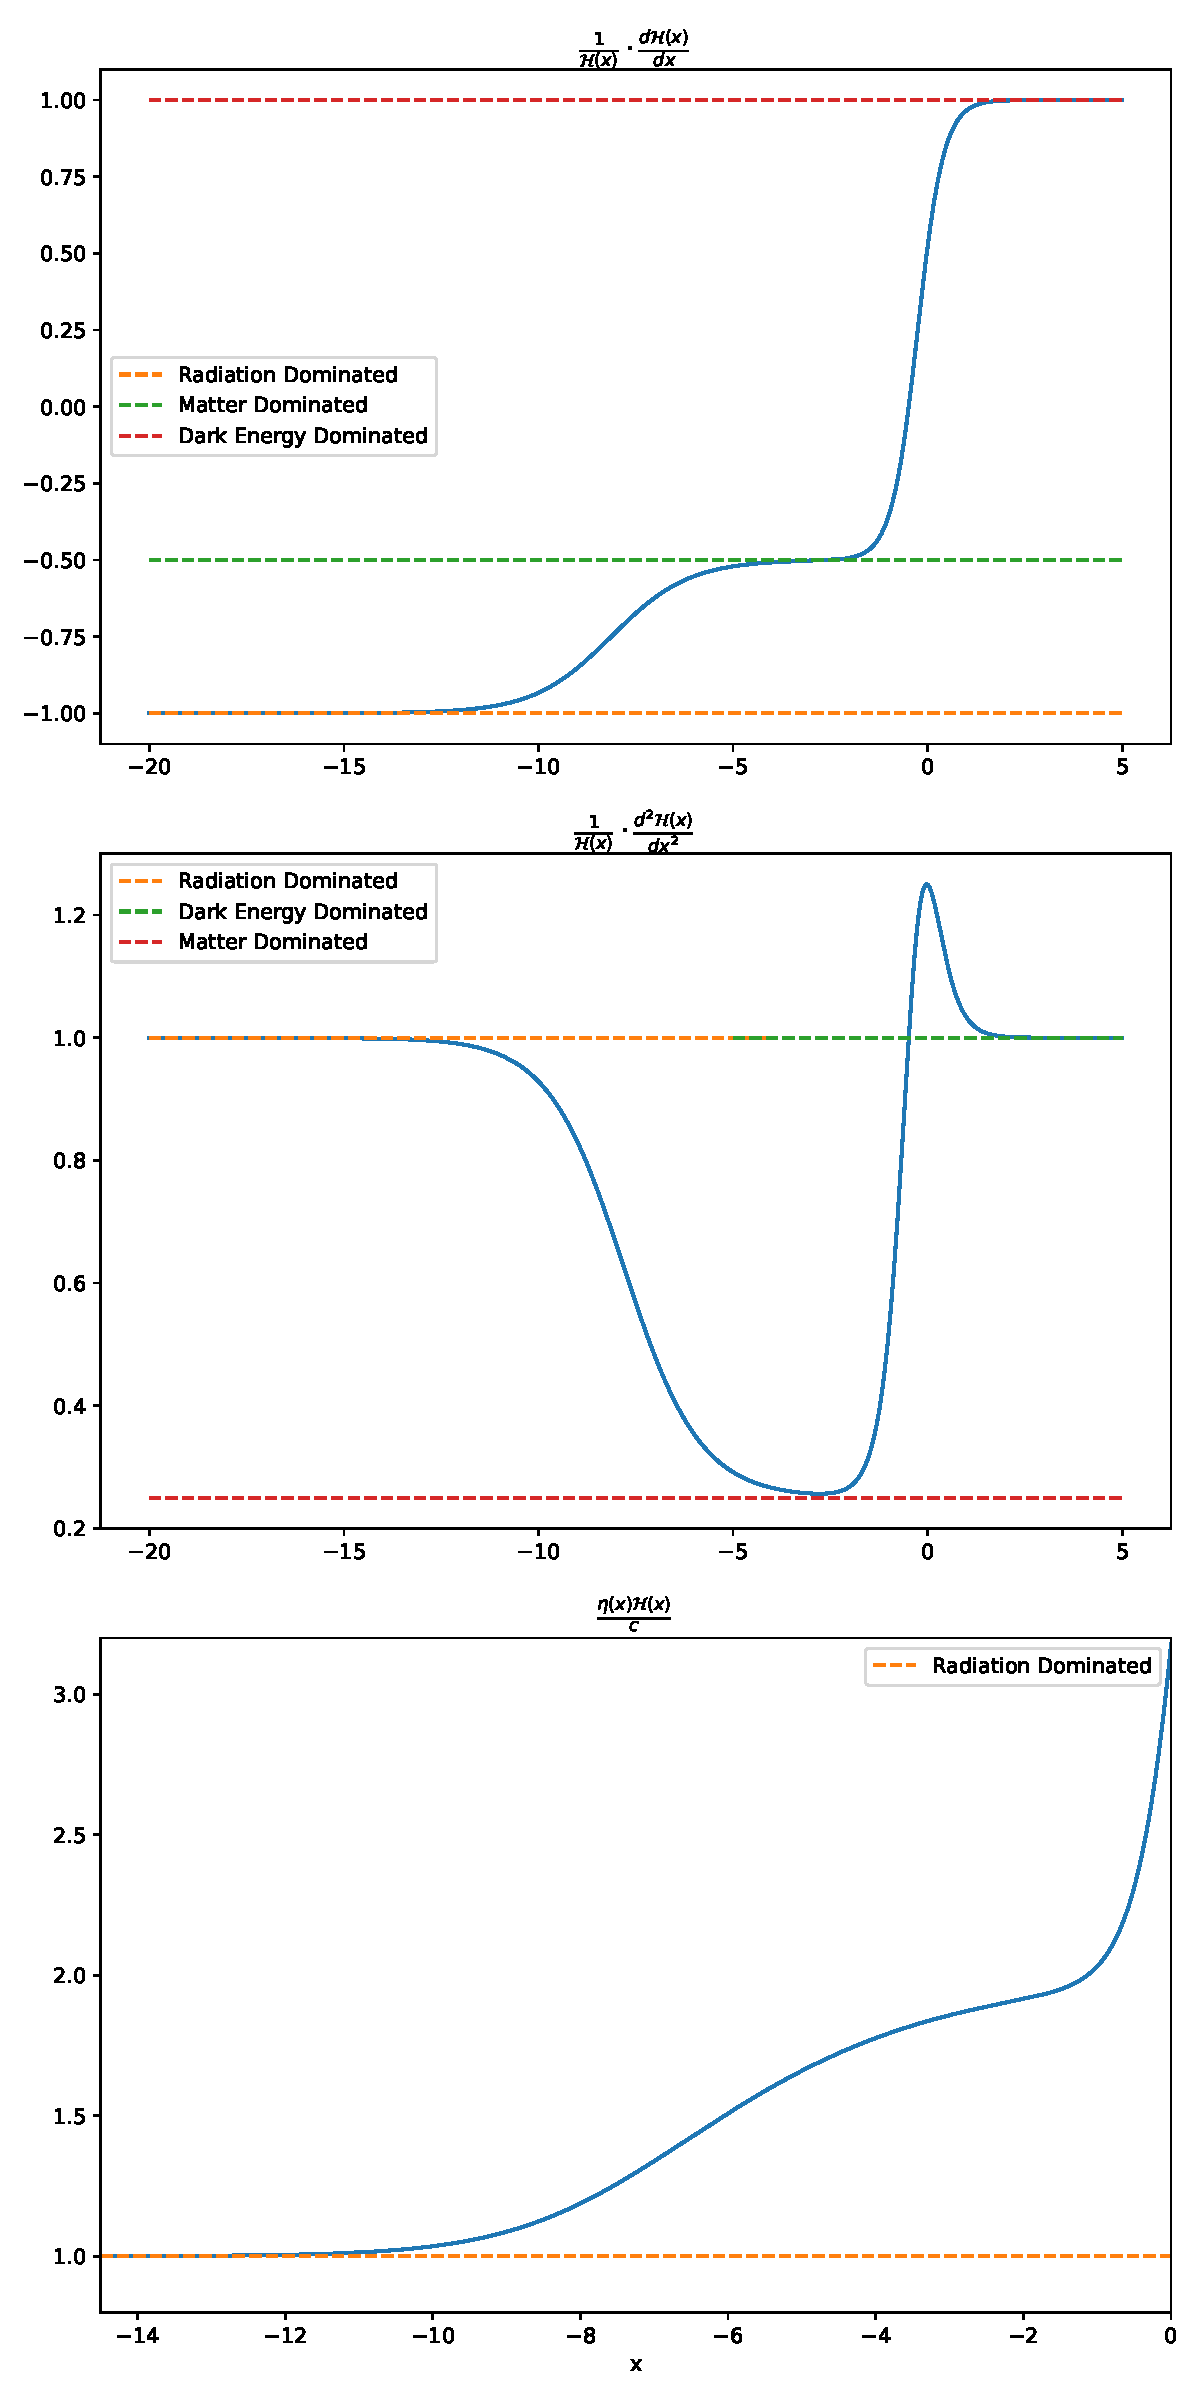
\includegraphics[scale=0.5]{../figures/milestone1/demonstrate_that_code_works.pdf}
   \caption{Plots to demonstrate that the code works properly. The dotted lines are the theoretical predictions.}\label{fig:M1_test_1}

\end{figure}



\subsection{Our results}



In figure \ref{fig:M1_Hp} we show a plot of the conformal Hubble parameter, $\mathcal{H}(x)$, which will often appear in calculations. $\mathcal{H}(x)$ is in actuality just $\dot{a}$, i.e. the rate of which the scale factor changes 
with respect to $x$. For two galaxies following the Hubble flow, the comoving distance, $d_\mathrm{comoving}$, is constant and equal to the physical distance today, since $d = a\cdot d_\mathrm{comoving}$.
The rate of change in the distance between them, $v$, is simply $v = \dot{a}\cdot d_\mathrm{comoving} = \mathcal{H}d_\mathrm{comoving} = Hd$, which is the Hubble law.
Since we study the FLRW universe, we know that massive particles follow the Hubble flow, so $v$ tells us firstly that at any given time, particles will move away from us 
twice as fast if they are twice as far away. Secondly, $\mathcal{H}(x)$ is, at any given time, the constant of proportionality for the first relation. In other words, $\mathcal{H}(x)$
is the expansion rate of the universe. In the plot, we see that this rate was largest at early times. We also see that the slope changes around radiation matter equality and around matter dark energy equality.
This can be understood by solving the Friedmann equation with one energy density component at a time. When dark energy becomes more dominant in the total energy density of the universe, the universe start to expand more rapidly again.
This is because the mass density has become too low for mass to be bound by "gravity". This happens at some time before matter dark energy equality as we can see
in the table \ref{tab:M1_times}.\\
\\
In figure \ref{fig:M1_t_x} we see the cosmic time, which is the time measured by an observer following the Hubble flow, plotted against $x$. The scale factor is proportional to $t^{1/2}$ during radiation domination, and proportional to $t^{2/3}$ during matter domination, \cite{Dodelson:MC}.
This explains why there is a change in the slope around radiation matter equality. As expected, the time today is of order giga years.\\
\\
In figure \ref{fig:M1_eta_x} we see the conformal time, $\eta(x)$. The conformal time, measured in length, is the distance light could have travelled, in comoving coordinates,
since the big bang. Measured in time, $\eta$ is then the amount of time light would have used to travel $\eta$ in length. The conversion factor between time and length is the speed of light.
Since $a=1$ today, $\eta(0)$ is then the size of the observable universe today, since light could have travelled those distances since the big bang. $\eta(x)$ is the comoving distance of causality.
The physical distance of causality at cosmic time, $t$, is then $a(t)\cdot \eta(x(t))$. The conformal time, in time, is larger than the cosmic time since the universe has expanded.
The expansion made all distances larger, and if we freeze the expansion, light would need more than 13.8 billion years to travel across the radius of the observable universe.
From table \ref{tab:M1_times} we see that light would need 46.3 billion years to travel this distance. Again we see that the slope changes around radiation matter equality, which is related to the change in $\mathcal{H}$.
The physical reason for why $\eta$ can change with respect to the cosmic time, is that the scale factor changes with time. If the scale factor is constant, $\eta$ will grow linearly. If the 
universe expands with the speed of light everywhere, $\eta$ will be constant, since light will not move relative to the comoving coordinates.\\
\\
In figure \ref{fig:M1_Omegas} we see how much each energy density parameter contributes to the sum of the energy density parameters. We see that the dark energy component
remains a small part of the total energy density in the universe until recently relative to the age of the universe. In the future, dark energy will be the only relevant density parameter,
so the universe will expand faster in the future compared to today. In the radiation dominated era, the universe was dominated by relativistic particles. As the universe
expanded and cooled down, the particles lost energy, and the energy content was dominated by non-relativistic matter. As the universe continued to expand, the mass density
decreases with the scale factor in all three spatial dimensions, i.e. $\rho \propto \frac{1}{a^3}$. Since the cosmological constant is constant everywhere, the total amount of dark energy
must increase when more space is created. This is observed close to $x=0$ in the plot.\\
\\
In figure \ref{fig:M1_data} we see that our model of the universe predicts a luminosity distance curve that agrees reasonably well with observations. This suggests that the universe is close to being flat.
In figure \ref{fig:M1_constraints} we see the $1\sigma$ and $2\sigma$ constraints from MCMC fits to supernova data in the $\Omega_\Lambda$ vs. $\Omega_M$ plane. 
The average value of the small Hubble parameter was $h= 0.70$ with $1\sigma = 0.0064$. We allowed curvature when fitting the data, and our best fit suggests, with $\chi^2=29.28$, that the curvature density parameter, $\Omega_K$,
is equal to 0.11.  


%by the scale factor, so it will be smaller than $H$ except for today where $a = 1$. Large values of $\mathcal{H}$ tells us that the      



\begin{figure}[h!]
   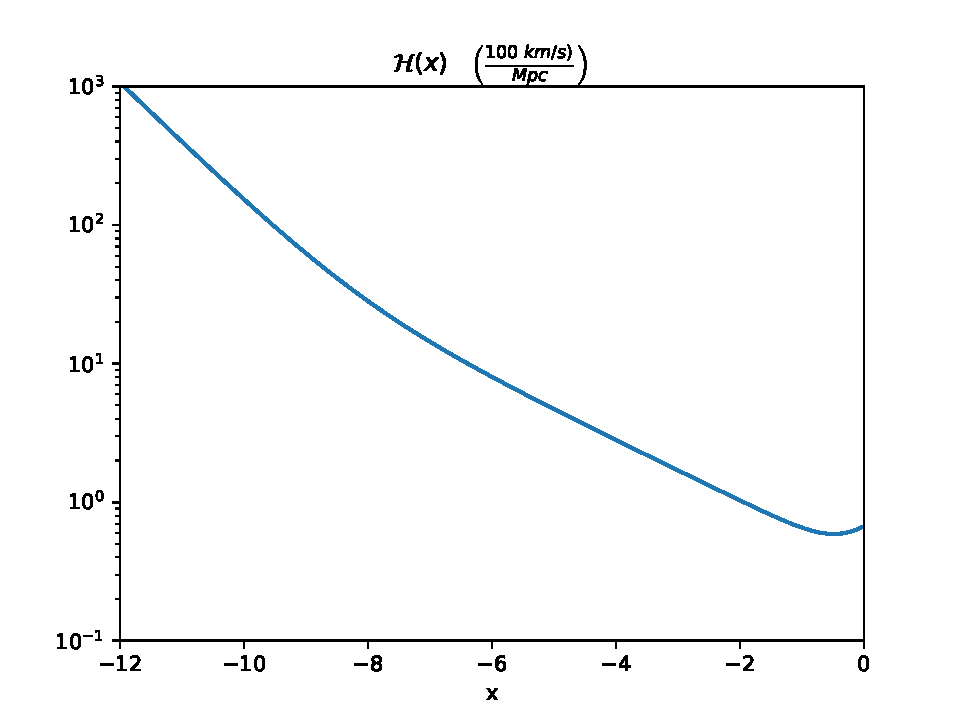
\includegraphics[scale=0.6]{../figures/milestone1/Hp_x.pdf}
   \caption{The conformal Hubble parameter as a function of $x$.}\label{fig:M1_Hp}
\end{figure}

\begin{figure}[h!]
   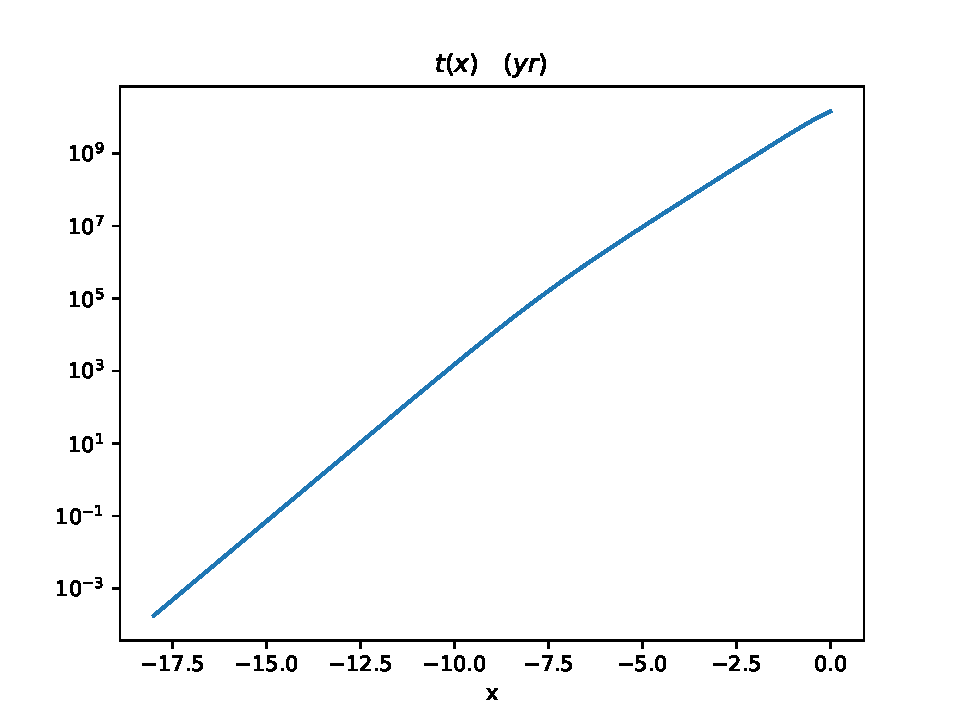
\includegraphics[scale=0.6]{../figures/milestone1/t_x.pdf}
   \caption{The cosmic time as a function of $x$.}\label{fig:M1_t_x}
\end{figure}

\begin{figure}[h!]
   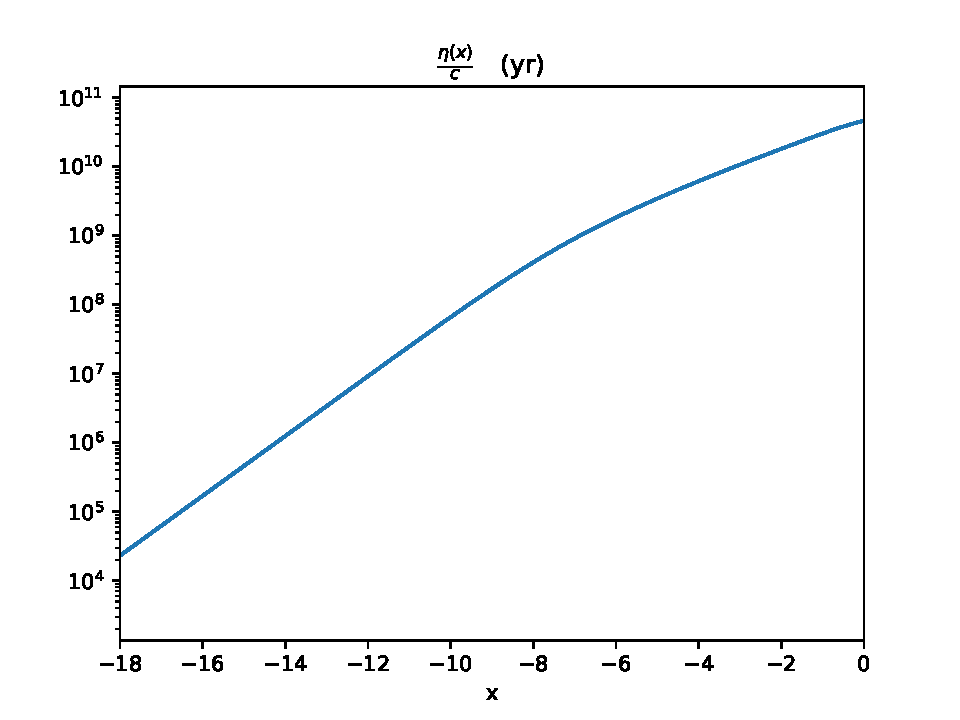
\includegraphics[scale=0.6]{../figures/milestone1/eta_x.pdf}
   \caption{The conformal time as a function of $x$.}\label{fig:M1_eta_x}
\end{figure}

\begin{figure}[h!]
   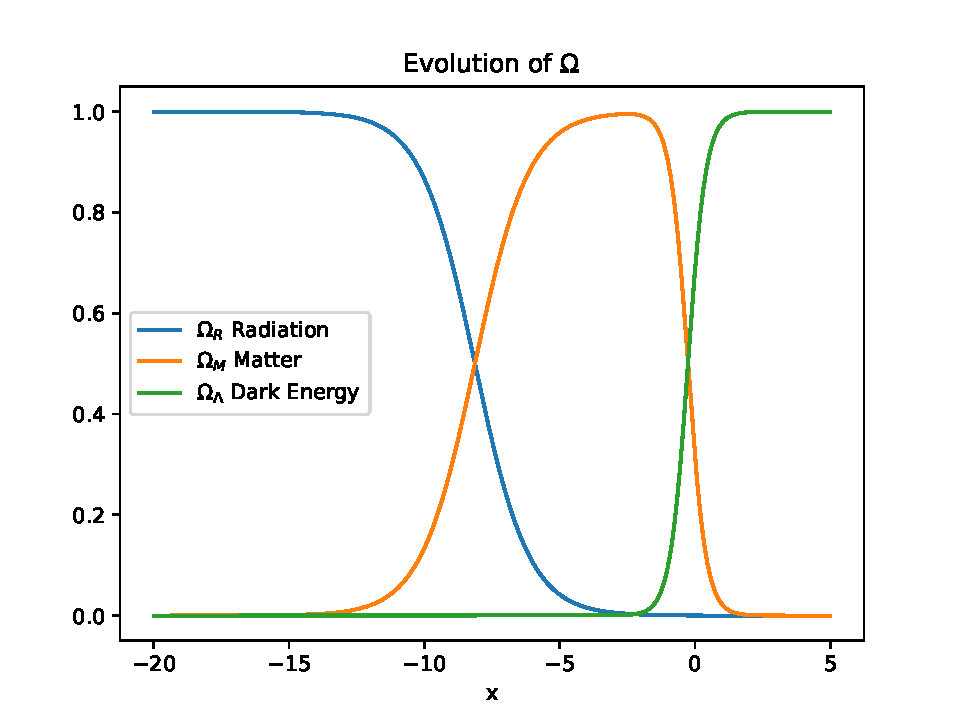
\includegraphics[scale=0.6]{../figures/milestone1/Omegas.pdf}
   \caption{The density parameters as a function of $x$.}\label{fig:M1_Omegas}
\end{figure}

\begin{figure}[h!]
   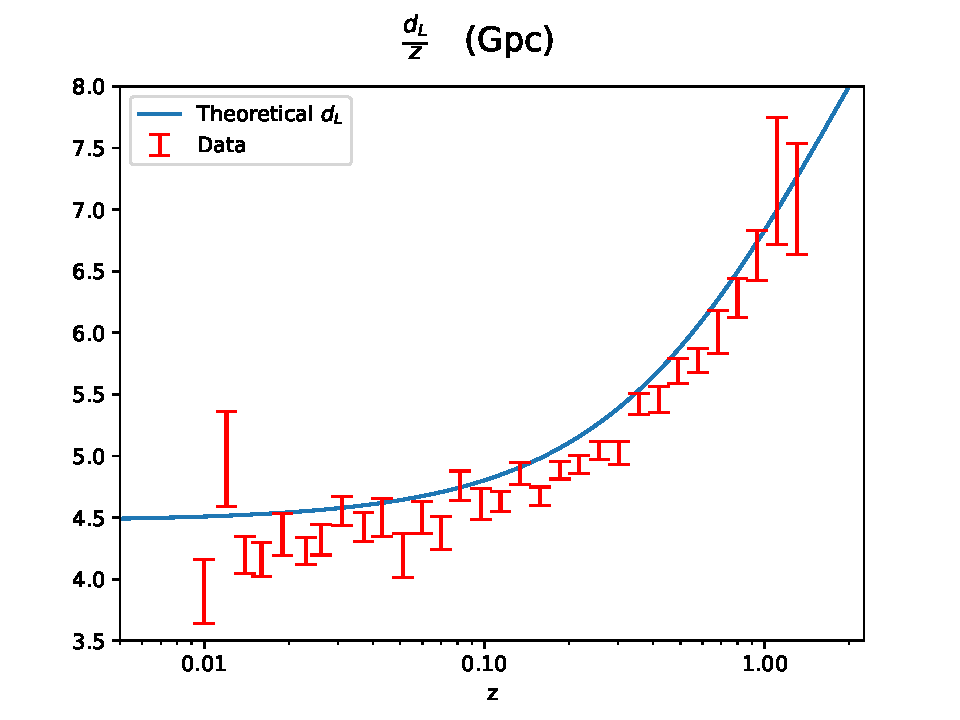
\includegraphics[scale=0.6]{../figures/milestone1/dataplot.pdf}
   \caption{The theoretical luminosity distance, divided by redshift, is plotted against redshift. Actual data from supernova observations is overplotted.}\label{fig:M1_data}
\end{figure}

\begin{figure}[h!]
   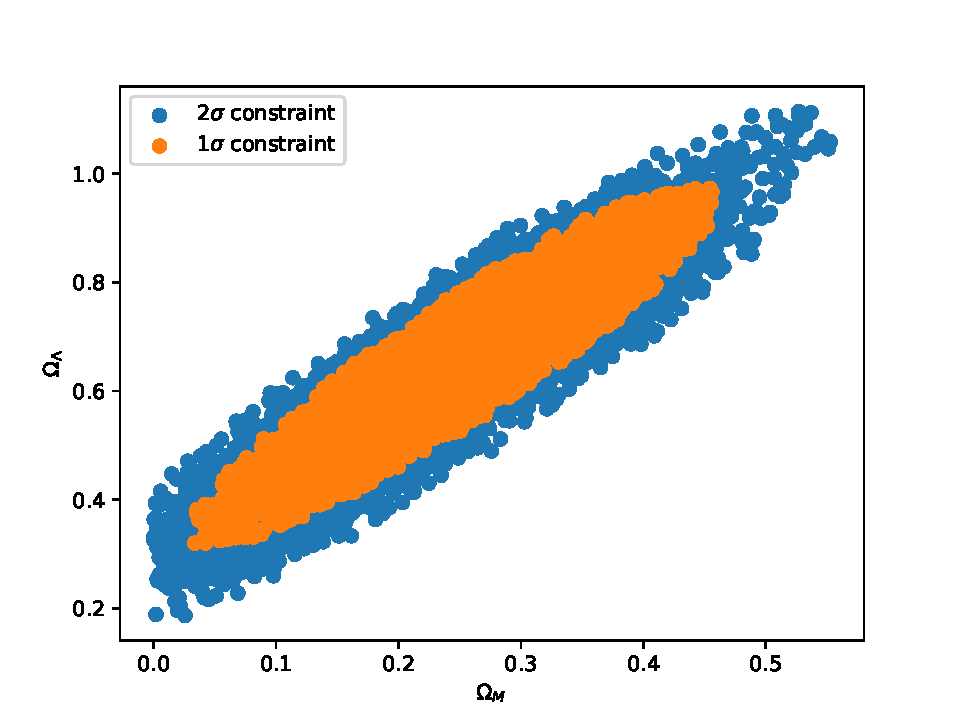
\includegraphics[scale=0.6]{../figures/milestone1/constraints.pdf}
   \caption{The $1\sigma$ and $2\sigma$ constraints from MCMC fits to supernova data in the $\Omega_\Lambda$ vs. $\Omega_M$ plane.}\label{fig:M1_constraints}
\end{figure}

\begin{figure}[h!]
   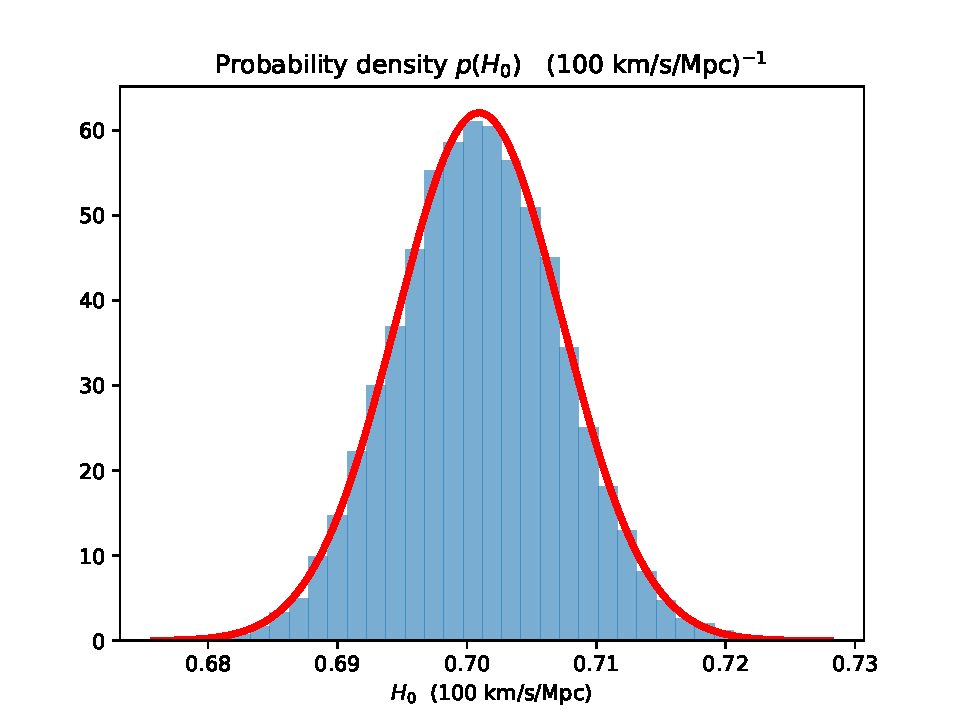
\includegraphics[scale=0.6]{../figures/milestone1/prob_dist_H0.pdf}
   \caption{The probability distribution of the Hubble parameter fitted with a Gaussian.}\label{fig:M1_prob_dist}
\end{figure}

\noindent
\\
In table \ref{tab:M1_times} we show some times for different events in the universe.
\begin{table}[h!] %%h! er for å tvinge tabellen til å være nærmest mulig her i dokumentet
   %\begin{center}
     \caption{Important times in cosmology stated in $x$, $z$ and $t$.} %Tabelltekst
     \label{tab:M1_times}
     \begin{tabular}{l|l|r|l} % for hver kolonne har du {a|b|c} der a er for 1.kolonne, b for 2. kolonne etc, l=venstrestil, r=høyrestilt, c = senterstilt. Se posisjonen til tallene i de forskjellige kolonnene. Har du 4 kolonner der alle er senterstilt blir det f.eks. {c|c|c|c}
       \textbf{Event} & \textbf{x, z, t}\\ %innhold i hver kolonne, legg til flere her hvis du har flere kolonner
       %(i) & (m) & (m/s)\\ %enheter for hver kolonne
       \hline %en horisontall linje for å skille overskriften fra tallene under. Vil du ha en slik linje mellom hver rad i tabellen så legg til en \hline mellom hver rad nedover her. Merk \\ er som vanlig linjeskift mens & skiller kolonner
       Radiation-Matter equality & -8.13,  3400.33, 51.06 [$10^3$ yr] \\
       Matter-Dark energy equality & -0.26, 0.29, 10.38 [Gyr]        \\
       Time of cosmic acceleration & -0.49, 0.63, 7.76 [Gyr]\\
       Age of the universe today & 0.00, 0.00, 13.86 [Gyr]  \\
       Conformal time today  & 1.90, -0.85, 46.32 [Gyr]\\

       %$Y_\mathrm{p}$ & 0\\
       \hline
     \end{tabular}
   %\end{center}
 \end{table}



\section{Milestone II}
Some introduction about what it is all about.

\subsection{Theory}
The theory behind this milestone.

\subsection{Implementation details}
Something about the numerical work.

\subsection{Results}
%Show and discuss the results.




%husk a snakke om tight coupling 
%husk a snakke om at vi løser fra radiation domination, men initial betingelsene er fra inflasjon p.g.a. horizon frys...
%sound hoizon vs. particle horizon
\section{Milestone III}
%Some introduction about what it is all about.
%In this milestone we look at 
In this milestone we calculate the evolution of the structures in the universe from after inflation until today.  In practice, this is done by 
solving the perturbed Einstein-Boltzmann equations numerically with initial conditions from inflation. This will give us the time evolution of the different physical quantities we are interested
in at different Fourier scales, $k$. We will go into more detail in the theory section. A detailed derivation of the relevant equations is given in \cite{winther:2023}. \\
\\
Since the observed CMB is a measurement of the photon temperature field today, it is of great interest for us to calculate the photon temperature fluctuations 
in the universe at all times and Fourier scales. These fluctuations can be evaluated today to reconstruct the CMB power spectrum we observe. 

\subsection{Theory}
%The theory behind this milestone.
%Boltzmann equations, spherical harmonics, perturbation theory...
Some regions in the early universe expanded more rapidly than others during inflation due to quantum fluctuations in the inflaton field, \cite{winther:2023}. These fluctuations
made the energy density of the universe inhomogeneous, which introduced fluctuations in the famous Friedmann-Lemaître-Robertson-Walker (FLRW) metric. We can find the initial conditions for the metric perturbations, $\Psi$ and $\Phi$, in the Newtonian gauge, and from there find the initial conditions for
the energy density perturbations of interest. This is done in \cite{winther:2023}.\\
\noindent
\\
The perturbations in the photon temperature field, $\delta T$, today are much smaller than the background temperature, $\overline{T}$. The same is true for the matter field on large scales.
This suggests that we can apply linear perturbation theory on the distribution functions and expect 
that the result will be valid today. The perturbed distribution functions, $f_i$, for baryons, photons and CDM take the form \[f_i(t,\vec{x},\vec{p})
 = \overline{f_i}(t,\vec{p}) + \delta f_i(t,\vec{x},\vec{p}),\] where $\overline{f_i}$ is the background distribution function and $\delta f_i$ is the perturbation. These perturbations will of course perturb the 
energy momentum tensor in the Einstein equations, which in turn will perturb the metric. This will then change how particles move through space and time, \cite{winther:2023}. We will therefore have a system of coupled differential equations.
The perturbed Einstein-Boltzmann equations can be solved in Fourier space with $x = \ln a$ as the time variable. The photon temperature perturbations, here defined as the relative perturbation $\Theta = \delta T/\overline{T}$, are expanded in Legendre multipoles,
such that we are left with multipoles, $\Theta_\ell$ of the photon distribution. Similarly, the CDM and baryon overdensities we solve for are defined as $\delta_\mathrm{CDM} = \frac{\delta \rho_{CDM}}{\overline{\rho}_{CDM}}$ and $\delta_\mathrm{b} = \frac{\delta \rho_{b}}{\overline{\rho}_{b}}$.
The velocities are defined similarly, such that they are dimensionless. We do not solve the equations for polarization, and neutrino perturbations are not included.\\ 
\\
The initial conditions:
$$
\boxed{
\begin{aligned}
\Psi &= -\frac{2}{3} \\
\Phi &= -\Psi \\
\delta_{\rm CDM} &= \delta_b = -\frac{3}{2} \Psi \\
v_{\rm CDM} &= v_b = -\frac{ck}{2\mathcal{H}} \Psi \\
&\text{Photons:}\\
\Theta_0 &= -\frac{1}{2} \Psi \\
\Theta_1 &= +\frac{ck}{6\mathcal{H}}\Psi \\
\Theta_2 &= -\frac{20ck}{45\mathcal{H}\tau^\prime} \Theta_1 \\
\Theta_\ell &= -\frac{\ell}{2\ell+1} \frac{ck}{\mathcal{H}\tau^\prime} \Theta_{\ell-1}\\
\end{aligned}
}
$$

The photon equations:
$$
\boxed{
\begin{aligned}
\Theta^\prime_0 &= -\frac{ck}{\mathcal{H}} \Theta_1 - \Phi^\prime, \\
\Theta^\prime_1 &=  \frac{ck}{3\mathcal{H}} \Theta_0 - \frac{2ck}{3\mathcal{H}}\Theta_2 +
\frac{ck}{3\mathcal{H}}\Psi + \tau^\prime\left[\Theta_1 + \frac{1}{3}v_b\right], \\
\Theta^\prime_\ell &= \frac{\ell ck}{(2\ell+1)\mathcal{H}}\Theta_{\ell-1} - \frac{(\ell+1)ck}{(2\ell+1)\mathcal{H}}
\Theta_{\ell+1} + \tau^\prime\left[\Theta_\ell - \frac{1}{10}\Theta_2
\delta_{\ell,2}\right],\\ 
& \mathrm{where} \ \ 2 \leq \ell \textless \ell_{\textrm{max}} \\
\Theta_{\ell}^\prime &= \frac{ck}{\mathcal{H}}
\Theta_{\ell-1}-c\frac{\ell+1}{\mathcal{H}\eta(x)}\Theta_\ell+\tau^\prime\Theta_\ell,
\quad\quad \ell = \ell_{\textrm{max}}\\
\end{aligned}
}
$$

Cold dark matter and baryons:
$$
\boxed{
\begin{aligned}
\delta_{\rm CDM}^\prime &= \frac{ck}{\mathcal{H}} v_{\rm CDM} - 3\Phi^\prime \\
v_{\rm CDM}^\prime &= -v_{\rm CDM} -\frac{ck}{\mathcal{H}} \Psi \\
\delta_b^\prime &= \frac{ck}{\mathcal{H}}v_b -3\Phi^\prime \\
v_b^\prime &= -v_b - \frac{ck}{\mathcal{H}}\Psi + \tau^\prime R(3\Theta_1 + v_b) \\
\end{aligned}
}
$$
Metric perturbations:
$$
\boxed{
\begin{aligned}
\Phi^\prime &= \Psi - \frac{c^2k^2}{3\mathcal{H}^2} \Phi\\
&+ \frac{H_0^2}{2\mathcal{H}^2}
\left[\Omega_{\rm CDM 0} a^{-1} \delta_{\rm CDM} + \Omega_{b 0} a^{-1} \delta_b + 4\Omega_{\gamma 0}
a^{-2}\Theta_0\right] \\
\Psi &= -\Phi - \frac{12H_0^2}{c^2k^2a^2}\left[\Omega_{\gamma 0}\Theta_2\right], \\
\end{aligned}
}
$$
where $R = \frac{4\Omega_{\gamma 0}}{3\Omega_{b 0} a}$. Some of these equations are numerically unstable early on, where the large value of $\tau^\prime$ is multiplied by the small value of $(3\Theta_1+v_b)$.  
This regime is known as the tight coupling regime, where the universe was opaque, and it can be related to time when the following three conditions hold simultaneously: $|\tau^\prime|>10$, $|\tau^\prime|>10\cdot \frac{ck}{\mathcal{H}}$ and
$x\leq -8.3$. The unstable equations are rewritten below.

$$
\boxed{
\begin{aligned}
q &= \frac{-[(1-R)\tau^\prime + (1+R)\tau^{\prime\prime}](3\Theta_1+v_b)}{(1+R)\tau^\prime + \frac{\mathcal{H}^\prime}{\mathcal{H}} -1}\\
  &\frac{-\frac{ck}{\mathcal{H}}\Psi + (1-\frac{\mathcal{H}^\prime}{\mathcal{H}})\frac{ck}{\mathcal{H}}(-\Theta_0 +
2\Theta_2) - \frac{ck}{\mathcal{H}}\Theta_0^\prime}{(1+R)\tau^\prime + \frac{\mathcal{H}^\prime}{\mathcal{H}} -1}\\
v_b^\prime &= \frac{1}{1+R} \left[-v_b - \frac{ck}{\mathcal{H}}\Psi + R(q +
\frac{ck}{\mathcal{H}}(-\Theta_0 + 2\Theta_2) - \frac{ck}{\mathcal{H}}\Psi)\right]\\
\Theta^\prime_1 &= \frac{1}{3} (q - v_b^\prime).
\end{aligned}
}
$$
The $2 \leq l$ photon multipoles in the tight coupling regime are given by the same expressions as in the initial conditions, but these multipoles are very small in this regime,
so we can simply set them to zero. The $\Theta_2$ multipole is calculated for numerical stability.\\
\\

 


\subsection{Implementation details}
We solved the differential equations in two different regimes and "sewed" the solutions together.
Since the last value in the first regime was used as an initial condition for the second regime, we removed the last value 
in the first regime, when "sewing" the solutions together, to remove the overlap between the solutions. A for loop was used to loop through all the Fourier scales, $k$, of interest.
The differential equations were solved using a Runge-Kutta 4 ODE solver. The solution was then splined with a 2D spline, since we have a complete solution in time for each $k$ value.\\ \\
Solutions of the background universe and the recombination history of the universe was also used.

\subsection{Results}
\subsubsection{Test results}
The code produces the following results with the cosmological test parameters given in table \ref{tab:test_parameters}. All the figures show plots at three different scales.
In figures \ref{fig:test1} and \ref{fig:test2} we see the density perturbation and the velocity, respectively, for both CDM and baryons. In figures \ref{fig:test3}
and \ref{fig:test4} we see the photon temperature monopole, $\Theta_0$, and the photon temperature dipole, $\Theta_1$, respectively. The gravitational potential, $\Phi$, is plotted
in figure \ref{fig:test5}. All plots seem to agree with the plots shown in \cite{winther:2023}.   


\begin{table}[h!] %%h! er for å tvinge tabellen til å være nærmest mulig her i dokumentet
   %\begin{center}
     \caption{Cosmological test parameters.} %Tabelltekst
     \label{tab:test_parameters}
     \begin{tabular}{l|l}%|r} % for hver kolonne har du {a|b|c} der a er for 1.kolonne, b for 2. kolonne etc, l=venstrestil, r=høyrestilt, c = senterstilt. Se posisjonen til tallene i de forskjellige kolonnene. Har du 4 kolonner der alle er senterstilt blir det f.eks. {c|c|c|c}
       \textbf{Parameter} & \textbf{Value}\\% & \textbf{Unit}\\ %innhold i hver kolonne, legg til flere her hvis du har flere kolonner
       %(i) & (m) & (m/s)\\ %enheter for hver kolonne
       \hline %en horisontall linje for å skille overskriften fra tallene under. Vil du ha en slik linje mellom hver rad i tabellen så legg til en \hline mellom hver rad nedover her. Merk \\ er som vanlig linjeskift mens & skiller kolonner
       $h$ & 0.7\\
       $\Omega_\mathrm{b}$ & 0.05\\
       $\Omega_\mathrm{CDM}$& 0.45\\
       $\Omega_\mathrm{\Lambda}$ & 0.5\\
       $\Omega_\mathrm{k}  $     & 0\\
       $\Omega_\mathrm{\nu}$ & 0\\
       $T_\mathrm{CMB}$ & 2.7255 $[K]$\\
       %$Y_\mathrm{p}$ & 0\\
       \hline
     \end{tabular}
   %\end{center}
 \end{table}

\begin{figure}[h!]
   %\hspace{-0.48cm}   
   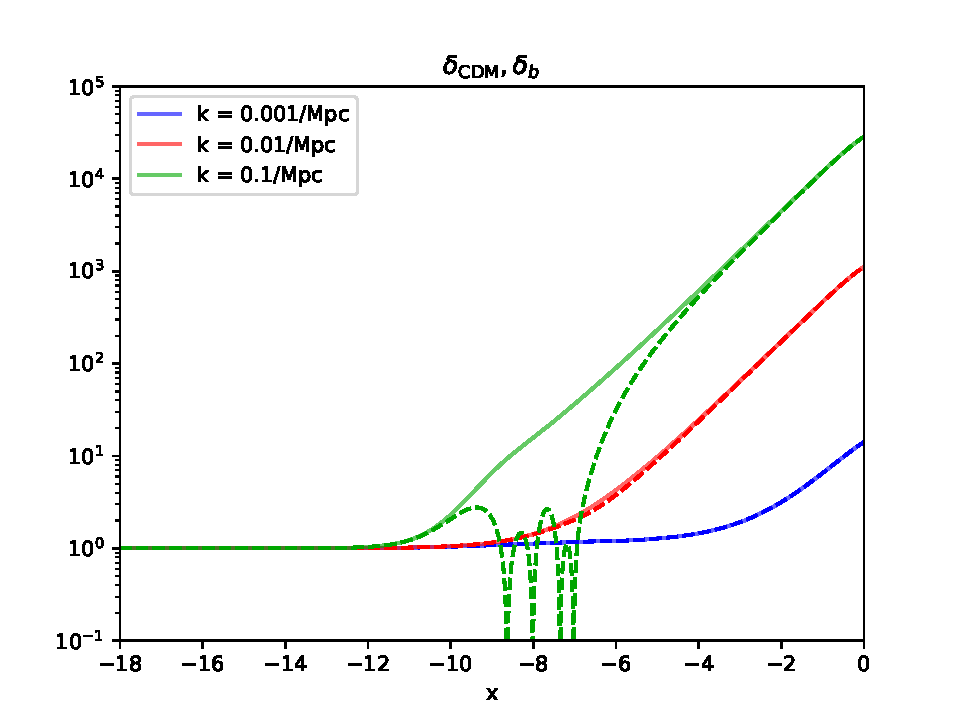
\includegraphics[scale=0.6]{../figures/milestone3/test_delta_cdm_delta_b.pdf}
   \caption{The CDM overdensity, in solid lines, and the absolute value of the baryon overdensity,
    in dotted lines, are plotted at different scales, $k$.}\label{fig:test1}
\end{figure}

\begin{figure}[h!]
   %\hspace{-0.48cm}   
   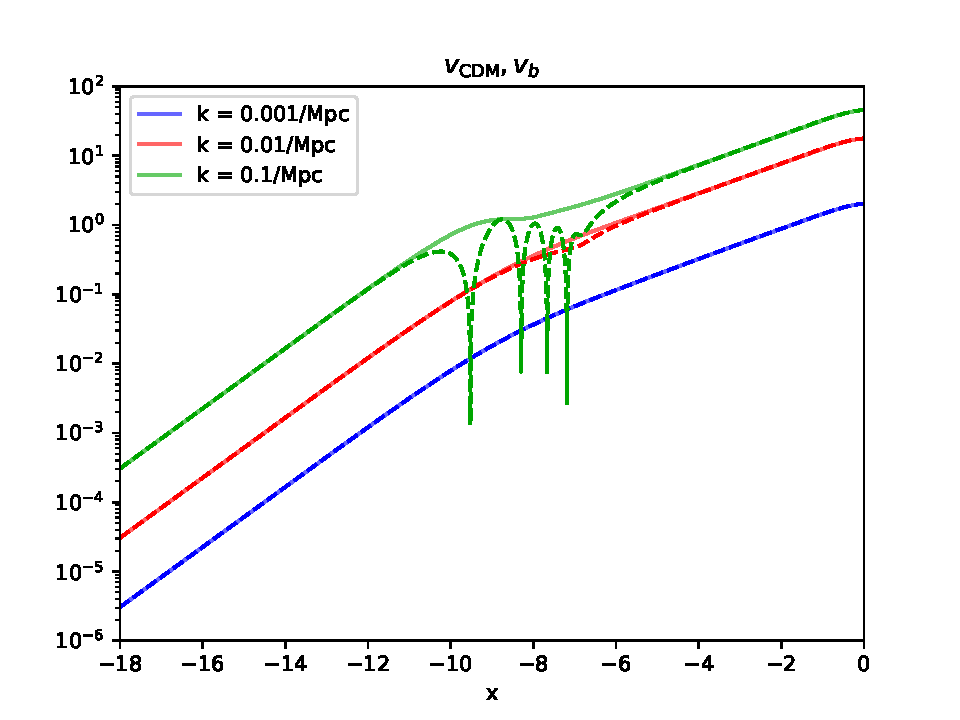
\includegraphics[scale=0.6]{../figures/milestone3/test_v_cdm_v_b.pdf}
   \caption{The CDM velocities, in solid lines, and the absolute value of the baryon velocities,
    in dotted lines, are plotted at different scales, $k$.}\label{fig:test2}
\end{figure}


\begin{figure}[h!]
   %\hspace{-0.48cm}   
   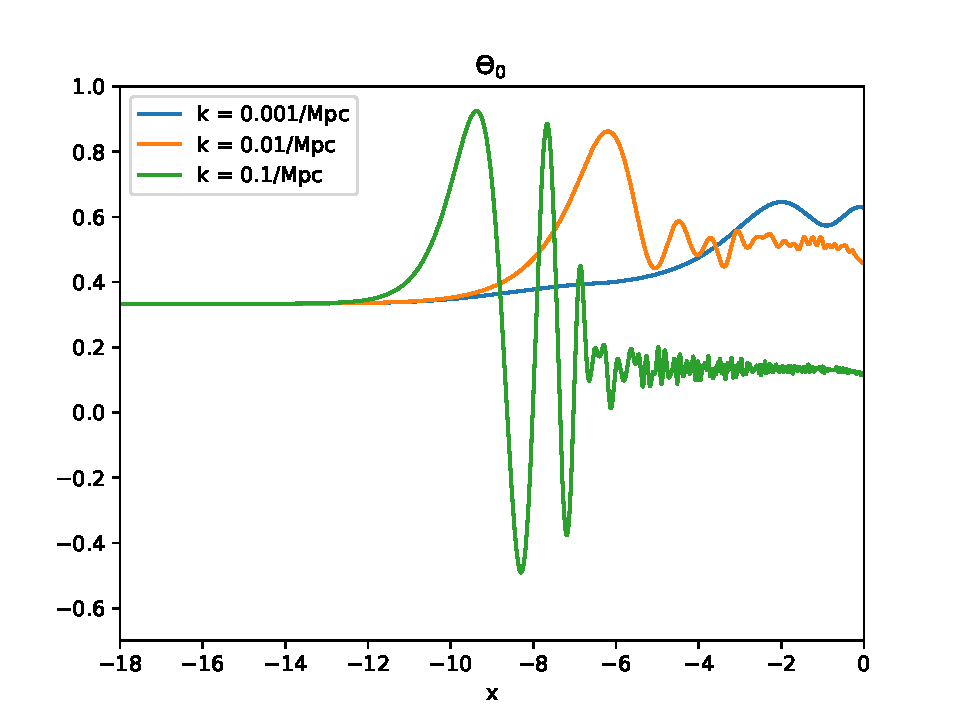
\includegraphics[scale=0.6]{../figures/milestone3/test_theta_0.pdf}
   \caption{The photon temperature monopole, $\Theta_0$, at different scales, $k$.}\label{fig:test3}
\end{figure}

\begin{figure}[h!]
   %\hspace{-0.48cm}   
   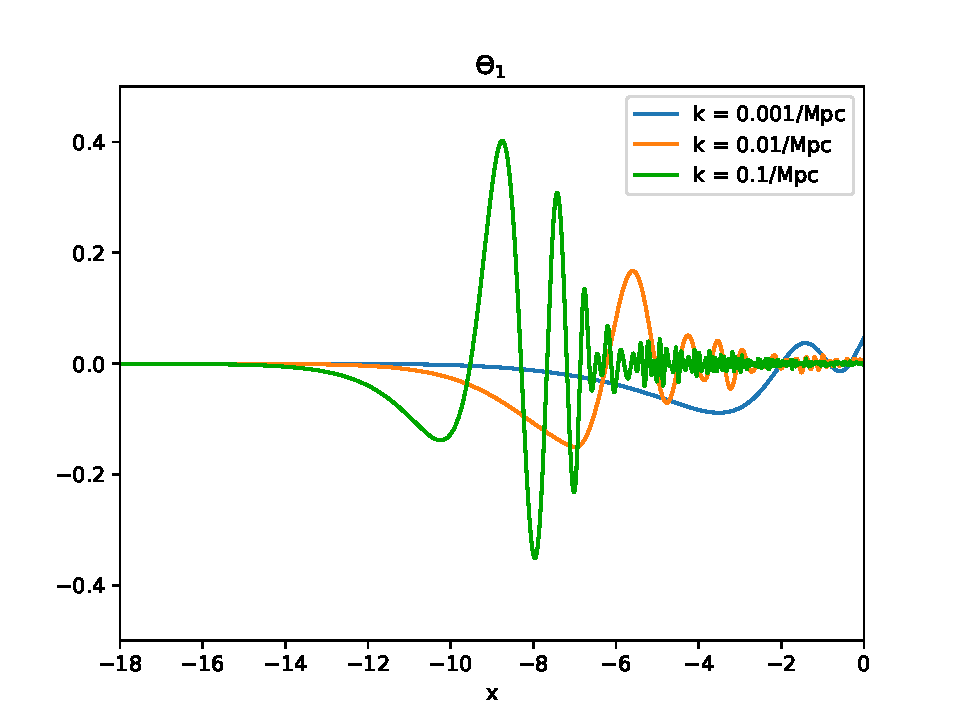
\includegraphics[scale=0.6]{../figures/milestone3/test_theta_1.pdf}
   \caption{The photon temperature dipole, $\Theta_1$, at different scales, $k$.}\label{fig:test4}
\end{figure}

\begin{figure}[h!]
   %\hspace{-0.48cm}   
   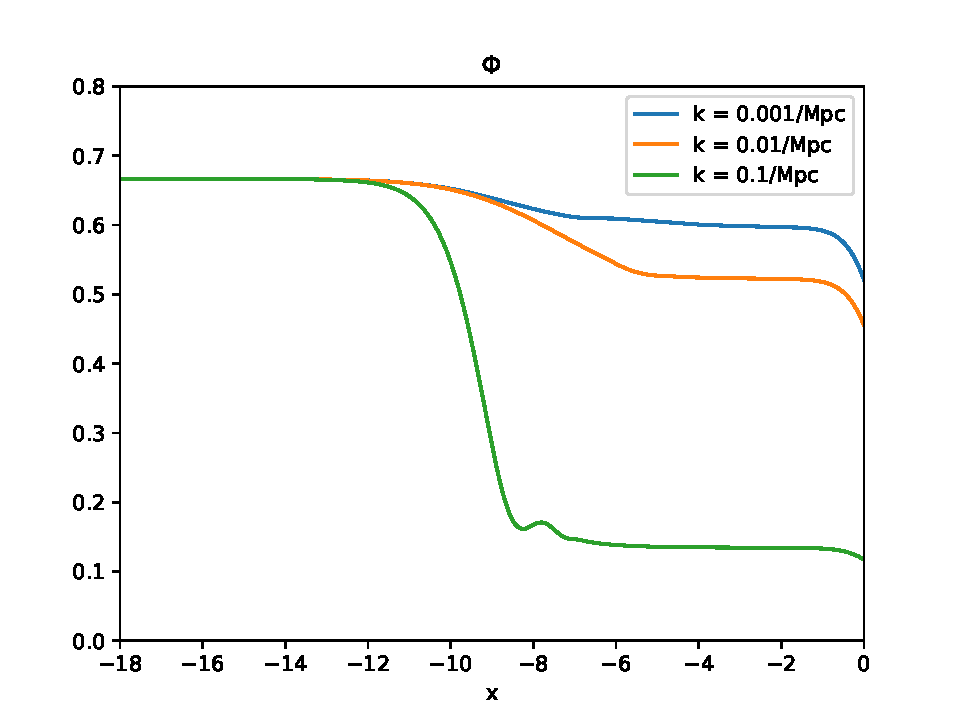
\includegraphics[scale=0.6]{../figures/milestone3/test_phi.pdf}
   \caption{The gravitational potential, $\Phi$, at different scales, $k$.}\label{fig:test5}
\end{figure}

\subsubsection{Results}
%theory section maybe???
% write about the slope of delta_cdm and compare to analytical result...all plots in general
In figure \ref{fig:delta_cdm_delta_b_zoom}, which is a zoomed in version of figure \ref{fig:delta_cdm_delta_b}, we see more clearly what is going on. Gravity travels with the same speed as light. This means that the conformal time, $\eta$,
gives us the maximum reach of gravity at any given time. Therefore, if the scale, $k$, of interest is larger than the conformal time, we should not see any correlation,
since the scale is causally disconnected. Using that Fourier modes enter the particle horizon when $k\eta=1$, we find
that the scale $k=10/\mathrm{Mpc}$ enters the particle horizon at $x\sim -15.4$.
We see that our results are consistent with the theory, as CDM clusters on this scale at $x\sim -16$. The reason why the overdensity oscillates, is because 
the mass is first compressed by gravity, then the pressure increases such that the mass rebounds. This process is then repeated until the Jeans mass is reached, where the Jeans mass is the mass needed to form structure.
Since the Jeans mass, in a static universe, depends linearly on the sound speed, we do not expect baryon structure to form in general before recombination, where the sound speed was $\sim c$, \cite{Shen:2022}. However, right after recombination  
the sound speed freezes out, and structures can more easily form. As recombination happened at $x=-7$, we can see in our results that the baryon overdensity starts to continously increase at this time. This supports the sound speed discussion.
For CDM we do not have any oscillating behavior at early times since CDM is pressureless and gravity only has to works against the cosmic acceleration.   
We note that the overdensity at some times is less than -1, which by definition is impossible. This is not a concern, since the quantities have not been scaled to represent physical values. 
\\ \\
In figure \ref{fig:v_cdm_v_b} we see that the oscillations in the baryonic overdensity has an expected corresponding oscillation in the baryonic fluid velocity, as the mass is contracting and rebounding repeatedly.
At a larger scale, seen in green, the mode enters the particle horizon later, and the baryonic overdensity undergoes fewer oscillation. For even larger scales, seen in 
red and blue, the modes enter the particle horizon after recombination, such that there are no oscillations.

%In figure \ref{fig:delta_gamma} the photon overdensity. 
%Velocity is negative right after perturbation has rebound

%Show and discuss the results.

\begin{figure}[h!]
   %\hspace{-0.48cm}   
   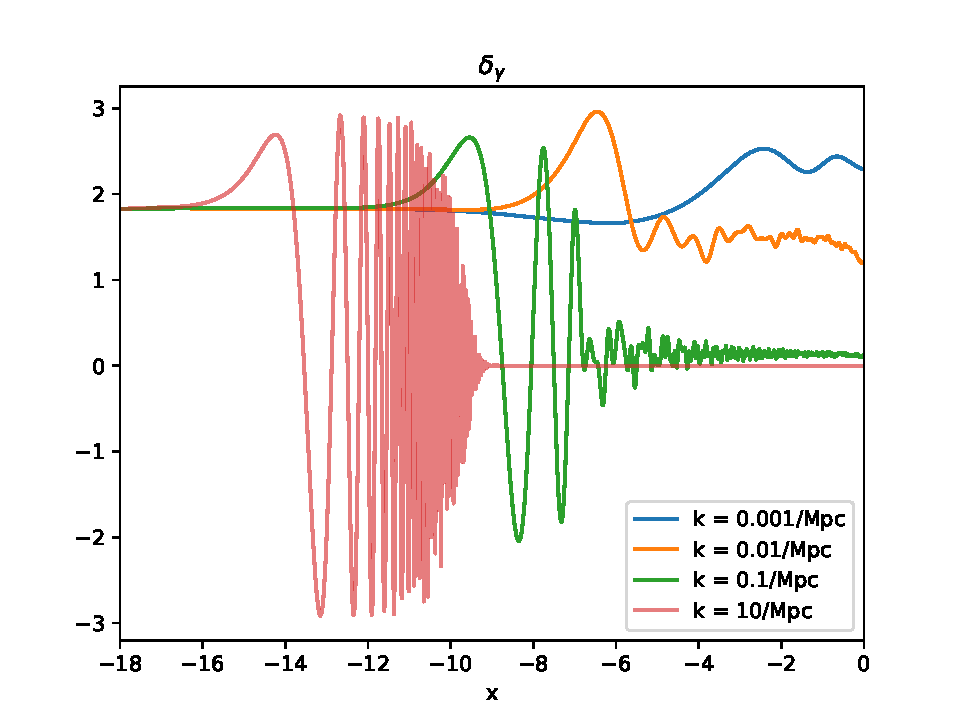
\includegraphics[scale=0.6]{../figures/milestone3/delta_gamma.pdf}
   \caption{The comparable photon overdensity, $\delta_\gamma = 4\Theta_0$, at four different scales, $k$. }\label{fig:delta_gamma}
\end{figure}

\begin{figure}[h!]
   %\hspace{-0.48cm}   
   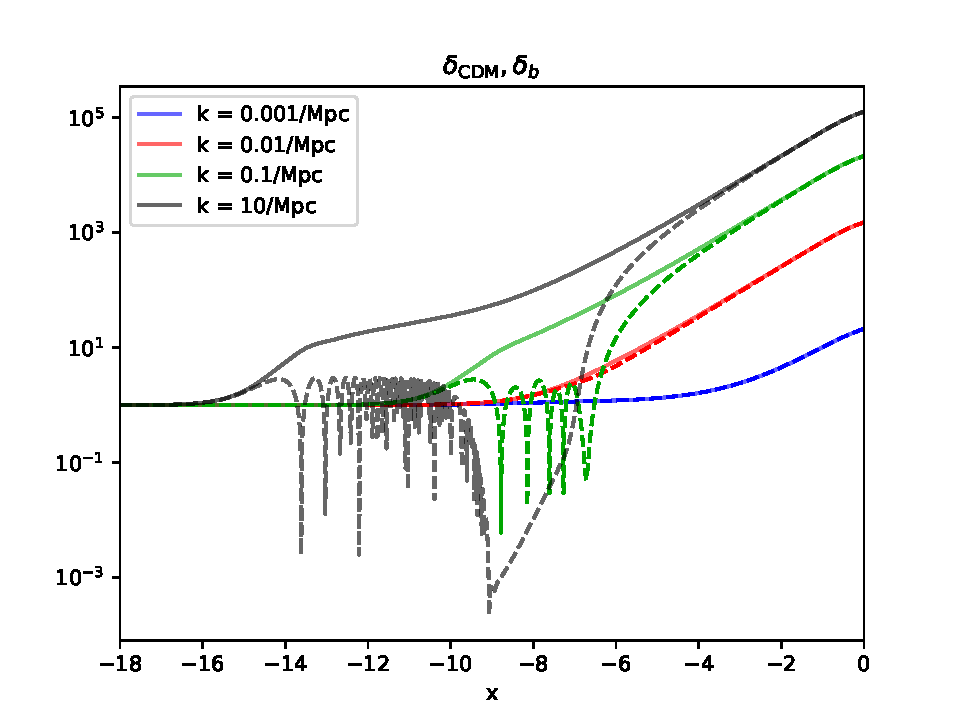
\includegraphics[scale=0.6]{../figures/milestone3/delta_cdm_delta_b.pdf}
   \caption{The CDM overdensity and the absolute value of the baryon overdensity plotted at four different scales, $k$. The solid lines are for CDM and the dotted lines are for baryons.}\label{fig:delta_cdm_delta_b}
\end{figure}

\begin{figure}[h!]
   %\hspace{-0.48cm}   
   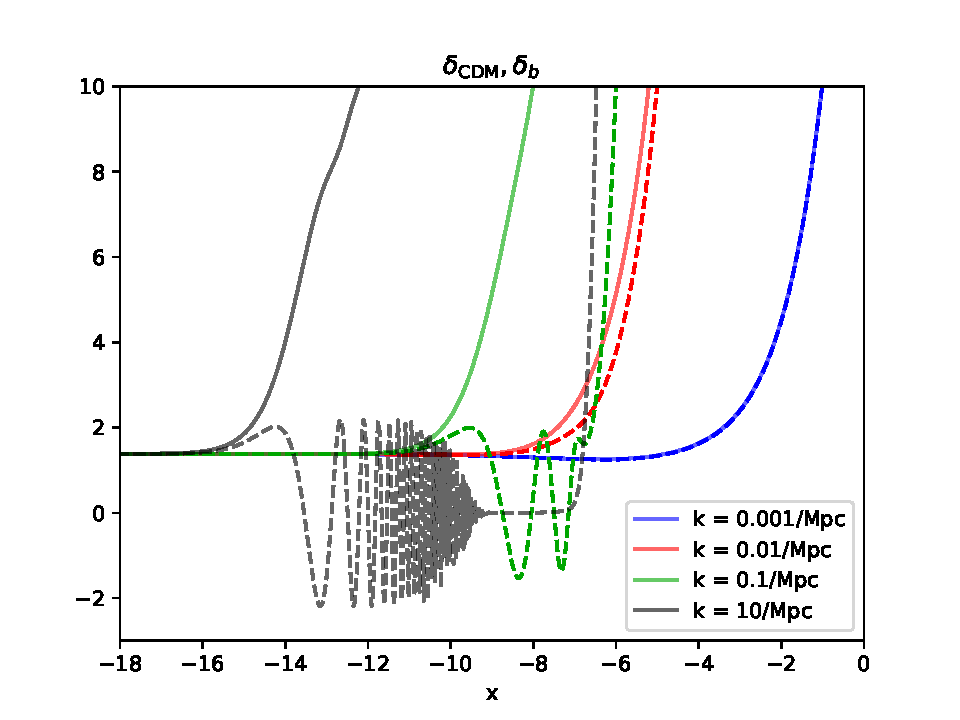
\includegraphics[scale=0.65]{../figures/milestone3/delta_cdm_delta_b_zoom.pdf}
   \caption{A closer look at figure \ref{fig:delta_cdm_delta_b} with linear y-scale and with the correct sign for the baryon overdensity.}\label{fig:delta_cdm_delta_b_zoom}
\end{figure}

\begin{figure}[h!]
   %\hspace{-0.48cm}   
   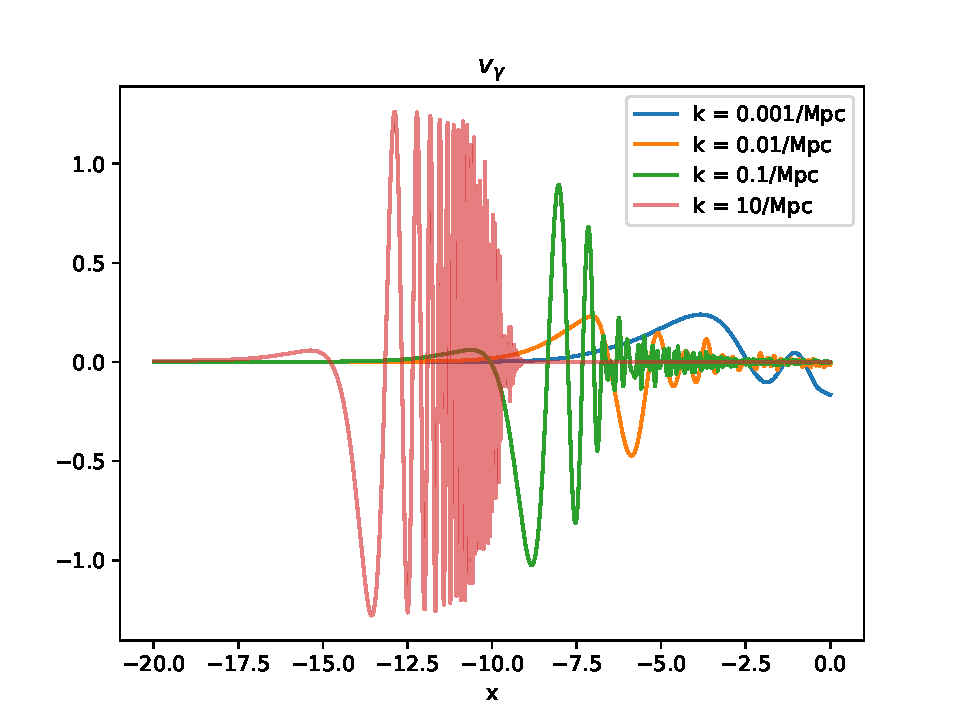
\includegraphics[scale=0.6]{../figures/milestone3/v_gamma.pdf}
   \caption{The photon velocity perturbation, $v_\gamma=-3\Theta_1$, at four different scales, $k$.}\label{fig:v_gamma}
\end{figure}

\begin{figure}[h!]
   %\hspace{-0.48cm}   
   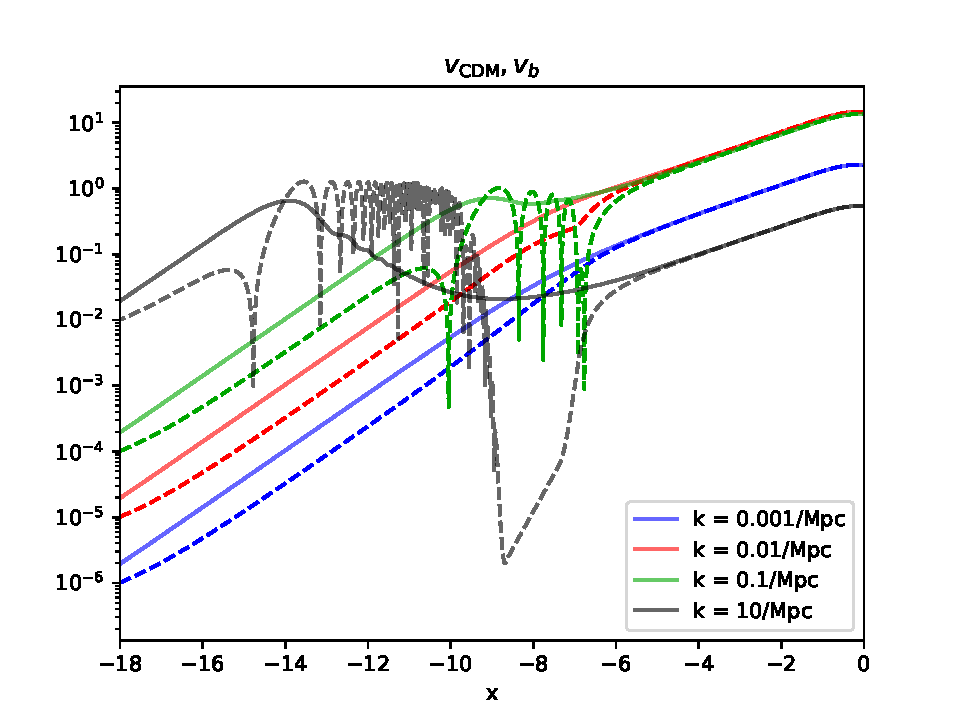
\includegraphics[scale=0.6]{../figures/milestone3/v_cdm_v_b.pdf}
   \caption{The CDM velocities, in solid lines, and the absolute value of the baryon velocities,
   in dotted lines, are plotted at four different scales, $k$.}\label{fig:v_cdm_v_b}
\end{figure}

\begin{figure}[h!]
   %\hspace{-0.48cm}   
   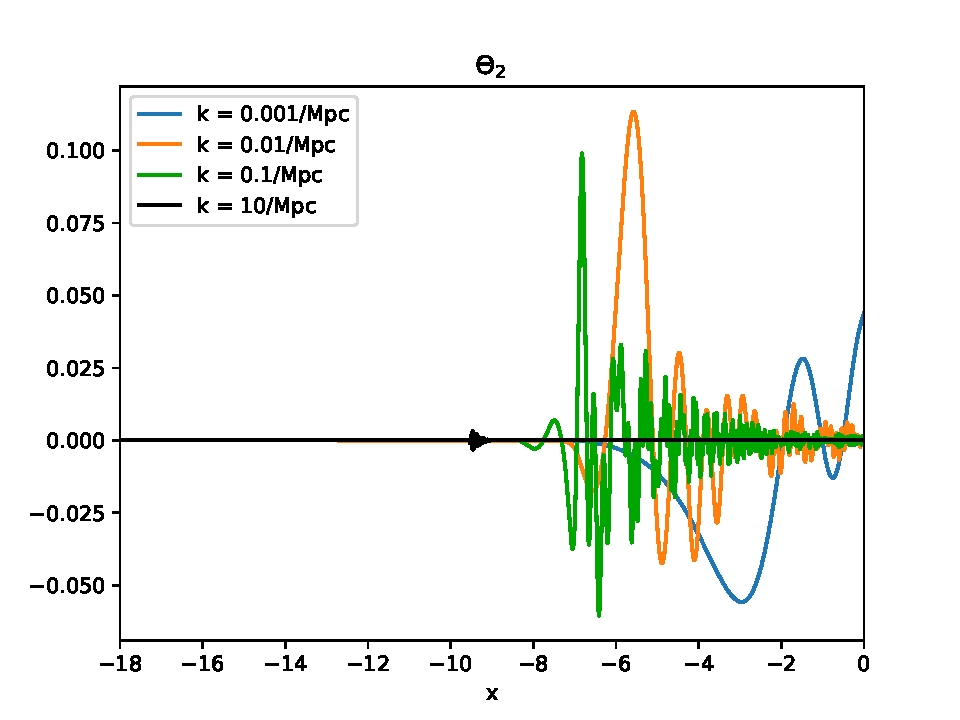
\includegraphics[scale=0.65]{../figures/milestone3/theta_2.pdf}
   \caption{The photon temperature quadrupole, $\Theta_2$, at four different scales, $k$.}\label{fig:theta2}
\end{figure}

\begin{figure}[h!]
   %\hspace{-0.48cm}   
   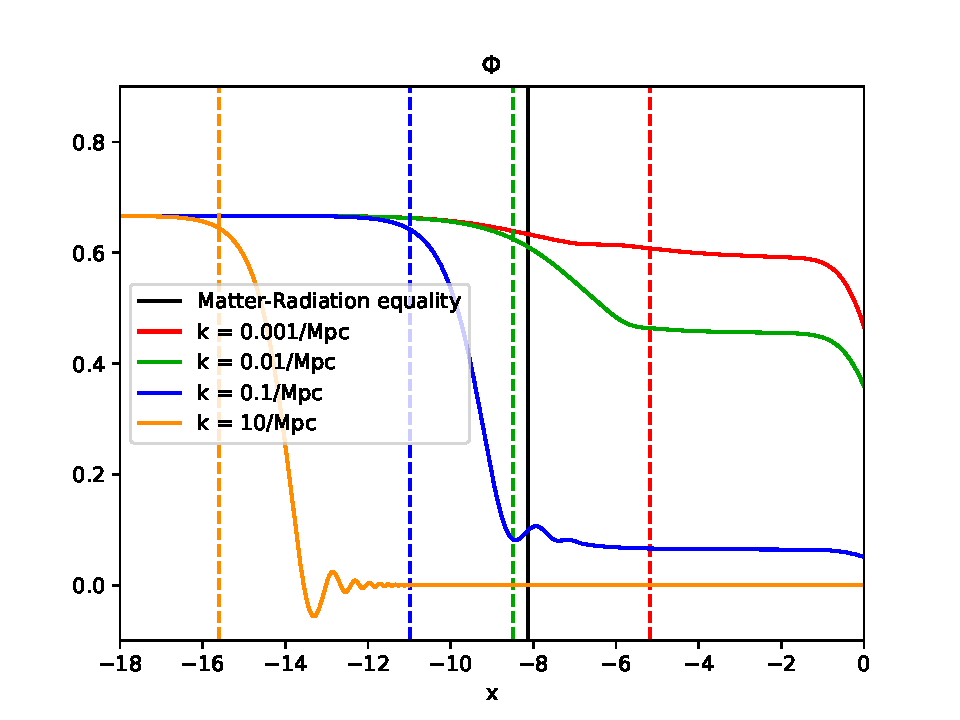
\includegraphics[scale=0.6]{../figures/milestone3/phi.pdf}
   \caption{The gravitational potential at four different scales, $k$.}\label{fig:phi}
\end{figure}

\begin{figure}[h!]
   %\hspace{-0.48cm}   
   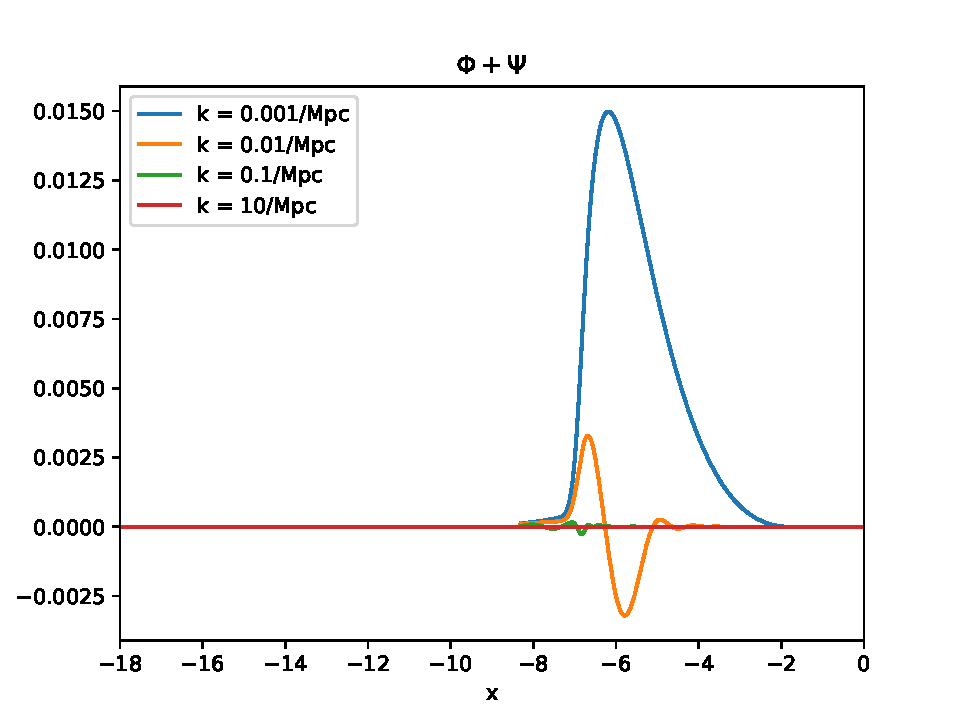
\includegraphics[scale=0.6]{../figures/milestone3/phi_psi.pdf}
   \caption{The sum of the two gravitational potentials, $\Phi$ and $\Psi$, at four different scales, $k$.}\label{fig:phi_psi}
\end{figure}



\section{Milestone IV}
Some introduction about what it is all about.

\subsection{Theory}
The theory behind this milestone.

\subsection{Implementation details}
Something about the numerical work.

\subsection{Results}
Show and discuss the results.

\section{Conclusions}

Write a short summary and conclusion in the end. 

%\begin{acknowledgements}
%      I thank my mom for financial support!!!
%\end{acknowledgements}

\bibliographystyle{aa} % style aa.bst
\bibliography{refs} % your references Yourfile.bib
%

%\bibliographystyle{plain} % We choose the "plain" reference style
%\section*{References}
%\bibliography{refs} % Entries are in the refs.bib file

%\begin{thebibliography}{}
%      \bibitem[1966]{baker} Baker, N. 1966,
%      in Stellar Evolution,
%      ed.\ R. F. Stein,\& A. G. W. Cameron
%      (Plenum, New York) 333
%
%      \bibitem[2023]{winther} Winther, H.A. 2023,
%      %\href{https://cmb.wintherscoming.no/milestone1.php}
%\end{thebibliography}

\end{document}